% !TEX root = ../main.tex
\section{How to accelerate cosmic particles?}

{\color{red}To be done}

% The presence of non-thermal particles is very common in the Universe: • Solar wind
% • Supernova remnants
% • Active galaxies
% • Gamma-Ray Bursts
% • Pulsar Wind Nebulae
% The presence of magnetized plasma is tightly connected to non-thermal particles.
%
%What we need is a system which satisfy these condition:
%
%\begin{itemize}
%\item \textbf{Large energetics}: we must take energy from somewhere! Kinetic energy translational in SNRs, roatitional in Pulsars, Gravitational energy in accretion disks, ...
%
%\item {Enough confinement time}: The particle has to stay in the accelerator for the time needed to accelerate it.
%
%\item {Lack of significant energy-losses}: Accelerating particles is useless if the loose energy too quickly.
%
%\item {A mechanism for energy transfer}: How to transfer energy from macroscopic objects into the (microscopic) acceleration of particles $\rightarrow$ we need to use electromagnetic.
%
%\end{itemize}
%
%While we have several candidates to supply the needed energy, having large scale, surving long enough, and with sufficiently low density, to solve the first three problems, the actual mechanism is trickier, and it was addressed for the first time by Enrico Fermin in 1949.
%
%Remember that all known acceleration mechanisms are electromagnetic in Nature. Since magnetic fields cannot make work on charged particles, one needs electric fields. 
%
%However, the only two possibilities are:
%%
%\begin{itemize}
%\item
%\textit{Regular acceleration}: we have that $\langle \vec{E} \rangle\neq 0$,  so we have to violate the conditions of ideal MHD,  which is very difficult.
%\item
%\textit{Stochastic acceleration}: in this case we respect the condition $\langle \vec{E}\rangle=0$,  but we have that $\langle \vec{E}^2\rangle\neq 0$.  This is the so called \textbf{second order Fermi acceleration}
%\end{itemize}

\section{Generalities of stochastic acceleration}

%%% CGPT
Consider a cyclic process in which particles gain energy, requiring a time \( \tau \) per cycle. Each cycle has an escape probability \( P_{\text{esc}} \) and an average fractional energy gain per cycle \( \xi \).

At each cycle, a particle with initial energy \( E_n \) has a probability \( 1-P_{\text{esc}} \) of being accelerated to \( E_{n+1} = (1 + \xi) E_n \). Thus, the energy of a cosmic particle after \( n \) acceleration cycles is:
%
\begin{equation}
E_n = E_0 (1 + \xi)^n
\end{equation}

The number of cycles needed to reach an energy \( E_n \) from an initial energy \( E_0 \) is given by:
%
\begin{equation}
n = \frac{\ln \left( E_n/E_0 \right)}{\ln (1 + \xi)}
\end{equation}

This implies that attaining higher energies requires a greater number of cycles.

Assuming a constant escape probability per encounter, the probability for a particle to remain in the acceleration region after \( n \) encounters is \( (1-P_{\text{esc}})^n \).

Over time, the cumulative fraction of particles with energies exceeding \( E \) can be computed using the sum of a geometric series with ratio \( x = (1-P_{\text{esc}}) \), leading to:
%
\begin{equation}
f(>E) 
\propto \sum_{m=n}^\infty (1 - P_{\rm esc})^m
= \frac{(1-P_{\text{esc}})^n}{P_{\text{esc}}} = \frac{(1-P_{\text{esc}})^{\frac{\ln \left( E_n/E_0 \right)}{\ln (1 + \xi)}}}{P_{\text{esc}}} 
\end{equation}

By utilizing the identity \( a^{\ln b} = b^{\ln a} \), we arrive at:
%
\begin{remark}
\begin{equation}\label{Eq:slopegeneralized}
f (>E) \propto \frac{1}{P_{\text{esc}}} \left( \frac{E}{E_0} \right)^{\gamma} \,\,\, \text{where} \,\,\, \gamma = \frac{\ln (1-P_{\text{esc}})}{\ln (1+\xi)} \simeq -\frac{P_{\text{esc}}}{\xi}
\end{equation}
\end{remark}

Here we used the approximation, \( \xi \ll 1 \) and \( P_{\text{esc}} \ll 1 \). Notice that this approach results in a power-law distribution for both first- and second-order Fermi mechanisms.

The maximum energy achievable in this statistical model is constrained by the finite lifetime of the accelerator, corresponding to a maximum of \( n \sim T / \tau \) cycles. Another limiting factor could be an increase in the escape probability with energy, such as in scenarios involving energy losses, which eventually counterbalances the energy gain.
%%% CGPT

\section{Second-Order Fermi Mechanism}

%%% CGPT
In 1949, Fermi proposed a physical system where this mechanism for particle acceleration can take place. In particular, he postulated the existence of an inhomogeneous interstellar medium, hence the presence of \emph{magnetic clouds} moving in random directions relative to the Galactic frame. These clouds, carrying magnetic fields, can reflect incoming charged particles.

The acceleration mechanism works as follows: \emph{particles gain energy when they encounter a magnetic cloud moving towards them and lose energy in encounters with clouds moving away}. {\color{red}Aggiungi plot.} Due to the greater frequency of head-on encounters compared to tail-on ones, there is an overall increase in energy.

To calculate the energy gain or loss per encounter, we use a double change of reference frame. We denote quantities in the cloud frame with primes and those in the Galactic frame without.

A test particle with initial energy \( E \) encounters a magnetic cloud moving with a velocity factor \( \beta = V/c \) along $x$. An observer on the cloud sees the following\footnote{In this context, we simplify for relativistic particles, thus \( p \simeq E \).
}:
%
\begin{equation}
E' = \gamma (E - \beta p_x) = \gamma E \left(1 - \beta \frac{p_x}{E} \right) = \gamma E \left(1 - \beta \mu_{\rm in} \right)
\end{equation}
%
where \( -1 \le \mu_{\rm in} \le 1 \) is the cosine of the angle between particle velocity and cloud velocity. 

Upon reflection by the cloud, the particle's energy, as observed externally, becomes:
%
\begin{equation}
E^{\prime\prime} 
= \gamma E^\prime (1+ \beta \mu^\prime_{\rm out}) 
= \gamma^2 E \left[ 1 - \beta \mu_{\rm in} + \beta \mu^\prime_{\rm out} - \beta^2 \mu_{\rm in} \mu^\prime_{\rm out} \right]
\end{equation}
%
clearly, if $\beta$ is the cloud velocity in the Galactic frame, $-\beta$ is the Galactic frame velocity with respect to the cloud.

Since magnetic fields do not perform work on the particles, the particle undergoes only elastic scattering within the cloud. This means its energy upon exiting the cloud remains unchanged in the cloud's frame of reference, represented as \( E'_f = E'_i \).

The relative change in energy is:
%
\begin{equation}
\frac{\Delta E}{E} = \frac{E'' - E}{E} =
\gamma^2  \left[ 1 - \beta \mu_{\rm in} + \beta \mu^\prime_{\rm out} - \beta^2 \mu_{\rm in} \mu^\prime_{\rm out} \right] - 1
%= \frac{ \beta^2 - \beta \mu_{\rm in} + \beta \mu^\prime_{\rm out} - \beta^2 \mu_{\rm in} \mu^\prime_{\rm out}}{1-\beta^2} 
%simeq 2\beta^2 + 2\beta \mu
\end{equation}

This result shows that the energy gain is proportional to the initial energy, meaning \( \Delta E/E \) is independent of \( E \).

It is crucial to recognize that both energy gain and loss are possible in this mechanism. This variability arises because the movements of both particles and magnetic clouds (consequently, the angles of interaction \( \mu \) and \( \mu' \)) are random. 
%
However, not all configurations are equally probable.

Given that a particle undergoes multiple scatterings off magnetic irregularities within the cloud, its exit direction becomes randomized, with an average \( \langle \mu'_{\rm out} \rangle = 0 \). Initially, we can average over the exit angle to get:
%
\begin{equation}
\left\langle \frac{\Delta E}{E} \right\rangle_{\mu^\prime} = 
\gamma^2 \left[ 1 - \beta \mu_{\rm in} \right] - 1
\end{equation}

Eventually, we must consider averaging over all possible initial angles. The rate at which a particle collides with a cloud is proportional to their relative velocity, leading to:
%
\begin{equation}
P(\mu) \propto v_{\rm{rel}} \propto 1 - \beta \mu_{\rm in} \rightarrow P(\mu) = \frac{1}{2} (1 - \beta \mu_{\rm in})
\end{equation}

Here we assumed \( v \approx c \) and we normalized so that the total probability equals one:
%
\begin{equation}
A \int_{-1}^{+1} d\mu (1 - \beta \mu) = 1 \rightarrow A = \frac{1}{2}
\end{equation}

Notice that \( \int_{\mu < 0} d\mu P(\mu) = 1 + \beta / 2 \) is larger than \( \int_{\mu > 0} d\mu P(\mu) = 1 - \beta/2 \), which means that \emph{head-on collisions} are more frequent compared to \emph{tail-on collisions}, which is the essence of Fermi’s acceleration mechanism.

Consequently, the average change in energy is given by:
%
\begin{remark}
\begin{equation}
\left\langle \frac{\Delta E}{E} \right\rangle_{\mu\mu'} 
= \int_{-1}^{+1} d\mu \, P(\mu) \left[ \gamma^2 \left( 1 - \beta \mu \right) - 1 \right] \simeq \frac{4}{3} \beta^2
\end{equation}
\end{remark}

Therefore, we have demonstrated that, on average, the energy variation in Fermi’s mechanism is \emph{positive}.
%
This confirms that Fermi's mechanism effectively accelerates charged particles. However, the average energy change is proportional only to \( \beta^2 \) underlining the \emph{stochastic nature} of the energy gain process.

Note that in this scheme the magnetic field's primary role is to alter the direction of particle motion, but the magnetic field itself does not provide the energy to increase the particle energy. Instead, the energy is supplied by an induced electric field~{\color{red}approfondisci}.

Considering \( \beta = u/c \), with \( u \sim v_A \sim 10 \) km/s, the fractional energy change per encounter \( \frac{\Delta E}{E} \) turns out to be around \( 10^{-8} \), indicating a rather inefficient acceleration process.

Indeed, for this mechanism to be a viable candidate for accelerating particles to the high energies observed in cosmic rays, it must do so efficiently.
%
Let's define the acceleration time, \( \tau_{\rm acc} \), as:
%
\begin{equation}
\tau_{\rm acc} = \left( \frac{1}{E} \frac{dE}{dt} \right)^{-1}
\end{equation}

Assuming a typical distance \( L \) between two clouds and no magnetic field in between (making our estimate a lower limit), the average time between two encounters is \( \tau_{\rm c} = L/c \).

Neglecting the time particles spend inside the cloud:
%
\begin{equation}
\frac{dE}{dt} \simeq \frac{\Delta E}{\tau_{\rm c}} = \frac{4}{3} \frac{\beta^2 c E}{L} \rightarrow \tau_{\rm acc} = \frac{3}{4} \frac{L}{c} \beta^{-2} 
\end{equation}

With typical values of \( \beta \sim 10^{-4} \) and \( L \sim 1 \) pc, it becomes evident that this mechanism would require nearly $\tau_{\rm acc} \sim $~Gyrs for a particle to double its energy. 
%
This timescale is far too long to explain the very high energies observed in Galactic cosmic rays.
In fact, energy losses in the ISM, such as ionization losses or spallation, typically occur more rapidly than the acceleration process postulated by Fermi, rendering the process even less efficient.

Moreover, the energy spectrum resulting from Fermi's original acceleration mechanism would depend on the ratio of $\tau_{\rm acc}$ to the energy-independent escape timescale $\tau_{\rm esc}$ (see Eq.~\ref{Eq:slopegeneralized}). {\color{red}Spiega meglio.}

This ratio is inherently unpredictable, as it varies based on the specific properties of the magnetic clouds and the regions where these clouds are densely concentrated. Consequently, different areas within the Galaxy could potentially accelerate cosmic rays with varying power law distributions. When combined, these contributions are unlikely to produce a singular, coherent power law spectrum akin to what is observed for Galactic cosmic rays on Earth.

This inconsistency is another drawback of the Fermi mechanism. In contrast, acceleration at shocks, which we will discuss next, circumvents both of these issues. 

Finally, we notice that although we do not believe that the bulk of cosmic-ray acceleration in our Galaxy is due to this mechanism, in several models of Galactic transport a similar mechanism is responsible of a tiny re-energization of the already accelerated cosmic rays.

%Furthermore, the energy gain does not depend on \( B \), the magnetic field strength. While the magnetic field mediates particle reflection, it does not directly appear in the Lorentz transformations.\todo{Approfondisci}

%As mentioned above, another possible way of working out the acceleration the to calculate the electric field seen in the Galactic frame by Lorentz transformation of the pure B field seen in the cloud frame. Since the two approaches must be equivalent the acceleration and the energy gain of the particle must also be independent of the cloud magnetic field in this case. This result is however far less intuitive with this approach.

\subsection{Second-order Fermi re-acceleration in the Fokker-Planck approach}

{\color{red}To be done}

%\begin{mdframed}
%\subsection*{Re-acceleration in the Fokker-Planck approach}
%
%Widely used for description of stochastic processes.
%%
%Let's define the probability that particle with momentum $\vb p$ at time $t$ changes momentum by $\Delta \vb p$ in time $\Delta t$.
%
%The phase space distribution function is $f(\vb x, \vb p, t)$ probability to find particle in phase space volume element d3xd3p.
%
%Using this defition
%%
%\begin{equation}
%f(\vb p, t+\Delta t) = 
%\int d^3(\Delta \vb p) \, f(\vb p - \Delta \vb p, t) P(\vb p - \Delta \vb p, \Delta \vb p)  
%\end{equation}
%
%Taylor expansion gives (to 2nd order in small $\Delta p$):
%%
%\begin{equation}
%f(\vb p, t) + \frac{\partial f}{\partial t} \Delta t \simeq \int d^3(\Delta \vb p) \, \left[ f P - \frac{\partial (fP)}{\partial p_i} \Delta p_i + \frac{1}{2} \frac{\partial^2 (fP)}{\partial p_i \partial p_j} \Delta p_i \Delta p_j + \dots \right]
%\end{equation}
%
%We impose now the normalization condition for the probability
%%
%\begin{equation}
%\int P(\vb p, \Delta \vb p) d^3 (\Delta p) = 1
%\end{equation}
%%
%and we define the Fokker-Planck coefficients as
%%
%\begin{eqnarray}
%\langle \Delta p_i \rangle & = & \int d^3 (\Delta p) P(\vb p, \Delta \vb p) \Delta p_i \\
%\langle \Delta p_i p_j \rangle&  = & \int d^3 (\Delta p) P(\vb p, \Delta \vb p) \Delta p_i \Delta p_j 
%\end{eqnarray}
%%
%which leads to
%%
%\begin{equation}
%\frac{\partial f}{\partial t} = 
%- \frac{\partial}{\partial p_i} \left( \frac{\langle \Delta p_i \rangle}{\Delta t} f \right) 
%+ \frac{1}{2} \frac{\partial^2}{\partial p_i \partial p_j} \left( \frac{\langle \Delta p_i \Delta p_j \rangle}{\Delta t} f \right)
%\end{equation}
%%
%with 1st term (rhs) describing systematic energy gain/losses, and 2nd diffu- sion part/dispersion/broadening.
%
%If scattering process is reversible in the sense that:
%%
%\begin{equation}
%P(\vb p, \Delta \vb p) = P(\vb p - \Delta \vb p, \Delta \vb p)
%\end{equation}
%
%\dots
%
%Fokker-Planck eq. then reduces to a diffusion equation in momentum space:
%%
%\begin{remark}
%\begin{equation}
%\frac{\partial f}{\partial t} = \frac{\partial}{\partial p_i} \left( D_{ij} \frac{\partial f}{\partial p_j} \right)
%\end{equation}
%\end{remark}
%%
%where $D_{ij}$ are the components of the diffusion tensor.
%\end{mdframed}

\section{First-Order Fermi Mechanism or Diffusive Shock Acceleration}

%%CGPT
The mechanism often associated with Fermi is, in fact, the result of the work by several authors, as Krymsky, Bell, Blandford, and Ostriker in the late 1970s. 
%
%Krymsky, G. F. Dokl. Akad. Nauk SSSR 243, 1306 (1977). 13. 
%Bell, A. R. M.N.R.A.S. 182, 147 (1978).
%Axford, W. I., Leer, E., and Skadron, G. Proc. 15th ICRC (Plovdiv) XI, 132 (1977). 15. 
%Blandford, R. D. & Ostriker, J. P. Astrophys. J. Lett. 221, L29 (1978).
%
They discovered that \emph{astrophysical shocks} could act as extremely efficient accelerators for cosmic particles, a process now known as \emph{diffusive shock acceleration (DSA)}.

Current observations confirm that particles are indeed accelerated at these shocks, evidenced by the radiation emitted from such regions, typically interpreted as the energy losses of accelerated electrons~{\color{red}mention the problem to identify hadronic signatures}.

We know at this point that, in the vicinity of the discontinuity, the upstream region is characterized by fast-moving, cold plasma, whereas the downstream region contains slower, hotter plasma. 
%
The typical shock wave's velocity in the ISM is approximately \( \sim 10^3-10^4 \) km/s, which corresponds to a Mach number of about 100-1000, placing us firmly in the strong shock regime.

The key concept here revolves around how particles perceive the plasma in the context of a shock front. From a particle's perspective, the plasma appears to approach at about the shock velocity from both the upstream and downstream sides.
%
Consider a group of particles with energy \( E \) initially located on the upstream side of the shock. These particles undergo diffusion through collisions with magnetic turbulence present in the plasma, which tends to isotropize their angular distribution in the frame where the upstream plasma is at rest.
%
Upon crossing the shock to the downstream side, these particles encounter magnetic turbulence associated with the downstream plasma. This plasma is moving towards the particles at a velocity \( \sim \frac{3}{4} u_s \) in the same reference frame. If collisions with the downstream plasma further isotropize the particles, then from the particles' viewpoint, they effectively experience a collision with a \emph{cloud} moving towards them. 
%
Some of these particles will eventually diffuse back to the upstream side of the shock. Upon their return, they perceive the upstream plasma as moving towards them, on average. In the shock frame, the unshocked plasma advances towards the downstream at a speed of \( |u_1 - u_2| \sim u_s \), resulting again in a head-on \emph{cloud} collision.
%
The continual diffusion of particles back and forth across the shock front invariably leads to increases in particle energy. Therefore, numerous cycles of crossing the shock can significantly accelerate the particles. 
%
As in both upstream and downstream scenarios, the particles experience head-on collisions, this mechanism will result in a  \emph{first-order} Fermi acceleration.


%Scattering ensures that once the particles enter in the upstream or downstream regions there their velocities become isotropically distributed.
%There are never crossings in which the particles lose energy, and the increment in energy is the same going in both directions.

It is clear from this description that, for this process to occur effectively, particle directions need to be isotropized, which can happen through pitch-angle scattering by MHD waves. The generation of these waves is attributed to large-scale turbulence cascade downstream, and upstream by the energetic particles themselves (cosmic-ray streaming).

Additionally, it's crucial for particles to have a finite probability of escaping downstream to fulfill the conditions of the generalized Fermi acceleration mechanism.

More quantitatively, consider now a test particle in the upstream with energy \( E \). This particle diffuses and crosses the shock, and its energy in the downstream \( E_d \) can be calculated using Lorentz transformation:
%
\begin{equation}
E_d = \gamma E (1 + \beta \mu)
\end{equation}
%
here, \( 0 \le \mu \le 1 \) and \( \beta = \frac{u_1 - u_2}{c} > 0 \).

The same principle applies to a particle transitioning from downstream to upstream, with the angle \( \mu^\prime \) having the opposite sign:
%
\begin{equation}
E_u = \gamma E_d (1 - \beta \mu^\prime)
\end{equation}
here, \( -1 \le \mu^\prime \le 0 \).

As a consequence, after completing a cycle (upstream $\rightarrow$ downstream $\rightarrow$ upstream), there is an overall gain in energy:
%
\begin{equation}
%= \gamma^2 E (1 + \beta \mu) (1 - \beta \mu^\prime) \rightarrow 
\frac{\Delta E}{E} = \frac{E_u - E}{E} = \gamma^2 (1 + \beta \mu) (1 - \beta \mu^\prime) - 1
\end{equation}

Notice that now, due to the different angular distributions, there are no configurations leading to an energy decrease, and \( \Delta E / E \) is \emph{always positive}.

To compute the mean energy gain over all the possible configurations, we have to compute the probability of a particle encountering the shock front with a specific pitch angle \( \mu \). 

Assuming \( n \) is the number density of isotropically distributed particles due to diffusion, this probability can be derived from the ratio of the flux of particles moving in the direction of \( \mu \) to the total flux \( J \):
%
\begin{equation}
J = \int d\Omega \frac{n}{4\pi} v \mu = \frac{n v}{4\pi} \int_0^{2\pi} d\phi \int_0^1 d\mu \mu = \frac{n v}{4}
\end{equation}
%
where we use the information that only those particles with a projected \( \cos \theta < 0 \) will actually cross the shock front.

Therefore, the probability density is given by:
%
\begin{equation}
P(\mu) \propto \frac{n \mu v}{J} = 4 \mu
\end{equation}

To normalize \( P \) as a probability, we impose the condition:
%
\begin{equation}
\int_0^1 d\mu P(\mu) = 1 \rightarrow P(\mu) = 2\mu 
\end{equation}

It is evident that this probability is symmetric in both directions. Consequently, the average energy gain can be calculated as follows:
%
\begin{remark}
\begin{equation}
\left\langle \frac{E_u -E}{E} \right\rangle_{\mu,\mu^\prime} = -\int_0^1 d\mu \int_{-1}^0 d\mu^\prime P(\mu)P(\mu^\prime)\left[ \gamma^2(1+\beta\mu)(1-\beta\mu')-1 \right] = \frac{4}{3} \beta = \frac{4}{3} \frac{u_1-u_2}{c}
\end{equation}
\end{remark}

This result implies that the energy gain per cycle is first order in $\beta$ as expected, for interstellar shock the resulting energy gain is of the order of \( 10^{-2}-10^{-3} \), which is enormously more than the second order mechanism! 

In assessing the efficiency of the proposed mechanism, we must additionally ensure that particles can effectively cross the shock in both directions. 
%
In the upstream region, particles, regardless of the diffusion coefficient, will eventually encounter the shock front, which moves towards them at thousands of kilometers per second. Hence, the probability of crossing from upstream to downstream, \( P_{1 \rightarrow 2} \), is 1. Particles leave the upstream region only when their Larmor radius becomes larger than the accelerator's size or the maximum scale of the upstream turbulence.

In the downstream region, besides diffusion, we must consider that the plasma moves away from the shock, dragging particles with it. This leads to a finite probability of particles not returning to the shock front, resulting in a leakage. To estimate this escape probability, we recall that the particle flux through an infinite planar shock is \( n v / 4 \), assuming efficient isotropization in the upstream. In the shock rest frame, there is a particle flow \( u_2 n \) downstream, away from the shock front, which is lost to the acceleration process. Therefore, the escape probability is:
%
\begin{equation}
P_{2 \rightarrow \infty} = \frac{4 u_2}{c}
\end{equation}

The probability of return to the shock front is simply:
%
\begin{equation}
P_{2 \rightarrow 1} = 1 - P_{2 \rightarrow \infty} = 1 - \frac{4 u_2}{c}
\end{equation}

With \( u_2/c \sim 10^{-2} \), most particles from the downstream will return to the upstream. This results in a highly efficient first-order Fermi acceleration mechanism with a high probability of completing a cycle.

The existence of a small escape probability is crucial, as it leads to a distribution of energies rather than uniform acceleration. Applying previous results, the slope of the \emph{differential spectrum}\footnote{The differential spectrum \( n(E)dE \) is  the number of particles with energy between \( E \) and \( E + dE \) thus \( E n(E) \propto E^{-\gamma} \)} produced by shock acceleration is:
%
\begin{remark}
\begin{equation}
\gamma \simeq \frac{3 u_2}{u_1 - u_2} + 1 = \frac{r + 2}{r - 1} \rightarrow 2
\end{equation}
\end{remark}

We found that this mechanism results in a \emph{universal} power-law spectrum for strong shocks, as the slope depends only on the compression factor. Worth noticing, the accelerated spectrum is independent of the diffusion coefficient, which in turn depends on the poor-understood microphysics of particle-wave scattering.

On the other hand, the acceleration process's efficiency and the potential to accelerate particles to sufficiently high energies dramatically depend on the diffusion coefficient. 
%
To estimate the acceleration time, we need to consider the energy gain per crossing and the time taken for each crossing. %
The average distance traveled by a particle in each region is obtained by equating the diffusion length (\( l_{\text{d,i}} \simeq \sqrt{2 D_i t_i} \)) to the distance covered by the shock or the advected plasma.

The total cycle time is the sum of the times spent in the downstream and upstream\footnote{$
t_{\rm c, i} = \frac{\lambda_i}{\langle v_{x,i} \rangle} = \frac{\lambda_i}{-\int_0^{\pi/2} v_i \cos \theta d\cos\theta} = \frac{\lambda_i}{v_i / 2} \sim \frac{2\lambda_i}{c}$}:
%
\begin{equation}
t_{\text{cycle}} = \frac{\lambda_1^2}{D_1} + \frac{\lambda_2^2}{D_2} = \left(\frac{D_1}{u_1^2} + \frac{D_2}{u_2^2}\right)
\end{equation}

The characteristic acceleration timescale is then:
%
\begin{equation}
\tau_{\text{acc}} = \frac{3}{u_1 - u_2} \left( \frac{D_1}{u_1} + \frac{D_2}{u_2} \right)
\end{equation}

To compare this time with the age of the system, we use typical values for the upstream diffusion coefficient and the shock speed of a young SNR. For example, with \( D_1 \simeq 10^{28}~\text{cm}^2~\text{s}^{-1} (E/\text{GeV})^{1/2} \) and \( u_1 = 10^4 \) km/s, we find:
%
\begin{equation}
{\color{red}\tau_{\text{acc}} \simeq 1~\text{kyr}~(E/\text{GeV})^{1/2}}
\end{equation}

However, observations of particles accelerated up to 100 TeV in events like Tycho's supernova (age \( \sim 500 \) years) suggest that our estimates are off by orders of magnitude. Reconciling this discrepancy requires \emph{reducing} the diffusion coefficient, possibly through cosmic-ray induced plasma instabilities. This leads to an inherently non-linear problem, underscoring the complexity of particle acceleration in astrophysical shocks.

\section{Cosmic ray spectrum from diffusive shock acceleration}

%%% CGPT
Let's explore the shock acceleration mechanism further through the formalism of a transport equation. We define our particle distribution function in the reference frame of the shock as:
%
\begin{equation}
f = f(z, t, p)
\end{equation}

This function is defined such that the number density of particles is given by:
%
\begin{equation}
n(z, t, p) dp = f(z, t, p) d^3 \mathbf{p} = f(z, t, p) 4 \pi p^2 dp
\end{equation}

The transport equation governing the distribution \( f \) is:
%
\begin{equation}
\frac{\partial f}{\partial t} + u\frac{\partial f}{\partial z} - \frac{1}{3}\left(\frac{du}{dz}\right)p\frac{\partial f}{\partial p} = \frac{\partial}{\partial z}\left[D_{zz} \frac{\partial f}{\partial z}\right] + Q
\end{equation}

We pass now to characterise the \emph{injection term} \( Q(p) \). Without injection terms or a nonzero initial condition, the only solution to this transport equation is \( f(z, p, t) = 0 \) everywhere.

It's important to remind that the shock is collisionless and possesses a small but finite thickness, comparable to the Larmor radius of the thermal particles forming the shock. For typical shock velocities of a few thousand kilometers per second, the Larmor radius is around \( r_{\rm L} \sim 10^8 \) cm, which, although small, is significant in astrophysical systems.
%
The gas in the downstream of the shock is thermalized, meaning its momentum distribution is Maxwellian. High-energy particles near the shock surface, which are part of this distribution, may have a Larmor radius large enough to cross the shock. Once they do, they enter the Fermi acceleration process, start gaining energy, and deviate from the Maxwellian distribution. This process constitutes the \emph{particle injection mechanism}. The likelihood of crossing the shock decreases with distance from the shock, as a larger Larmor radius would be necessary. This justifies the assumption that particles are injected at the shock.

Consequently, we can represent the injection term as a delta-function in position:
%
\begin{equation}
Q(z, t, p) \propto \delta(z) \delta(p - p_{\text{inj}})
\end{equation}
%
where \( p_{\text{inj}} \) denotes the minimum momentum required for this process to occur.

By introducing \( Q_0 \) to normalize the fraction of the particle flux crossing the shock per unit volume in phase space:
%
\begin{equation}
\eta n_{\rm inj} u_1 = \int dz \, 4 \pi p^2 dp \, Q_0 \delta(z) \delta(p - p_{\text{inj}}) \rightarrow Q_0 = \eta \frac{n_{\rm inj} u_1}{4 \pi p^2_{\rm inj}}
\end{equation}
%
hence, the transport equation becomes:
%
\begin{equation}
\frac{\partial f}{\partial t} + u\frac{\partial f}{\partial z} - \frac{1}{3}\left(\frac{du}{dz}\right)p\frac{\partial f}{\partial p} = \frac{\partial}{\partial z}\left[D_{zz} \frac{\partial f}{\partial z}\right] + \delta(z) \delta(p-p_{\text{inj}})Q_0
\end{equation}

Assuming stationarity (\( \frac{\partial f}{\partial t} = 0 \)) and focusing on the upstream region where \( \frac{du}{dz} = 0 \), the equation becomes:
%
\begin{equation}
u \frac{\partial f}{\partial z} - \frac{\partial}{\partial z} \left[D \frac{\partial f}{\partial z}\right] = 0 \rightarrow \frac{\partial}{\partial z}\left[uf - D \frac{\partial f}{\partial z}\right] = 0
\end{equation}

This implies that the sum of the advective and diffusive fluxes, \( uf - D\frac{\partial f}{\partial z} \), must be constant. Since it's unphysical to have accelerated particles at infinity in the upstream direction, the flux at \( z = +\infty \) is zero, and thus this constant value must also be zero:
%
\begin{equation}
uf - D \frac{\partial f}{\partial z} = 0
\end{equation}

As an ansatz, we propose the following form for \( f \):
%
\begin{equation}
f = f_0 \exp\left(\alpha z\right)
\end{equation}

Substituting this into the equation, we obtain \( \alpha = \frac{u_1}{D} \), leading to the upstream distribution function:
%
\begin{equation}
f_{\rm u}(z, p) = f_0 \exp \left[ \frac{u_1 z}{D(p)} \right]
\end{equation}

Here, \( f_0 \) is the distribution function at the shock, serving as the boundary condition to solve the equation. The ratio \( \frac{D(p)}{u_1} \) is known as the \emph{typical diffusion length} of the plasma. This represents a balance point where the diffusion of particles away from the shock is counterbalanced by the plasma pushing them back towards the shock.

In the downstream region, the only plausible stationary solution is to assume that the particle distribution function \( f_{\text{d}} = f_0 \) remains constant in space. This constancy is necessary because the particle density cannot diverge at downstream infinity (as this would be unphysical), and it cannot decrease either. If it did, diffusion and advection would concurrently remove particles from the downstream region, violating the stationary assumption.

It's important to note that \( f \) is continuous across the shock. Unlike dynamic thermodynamic quantities, \( f \) is not a property of the plasma itself. The particles we're considering for acceleration have Larmor radii larger than the shock's thickness, meaning they do not \emph{feel} the discontinuity.

To determine \( f_0 \), we integrate the transport equation across the shock:
%
\begin{equation}
\lim_{\epsilon \rightarrow 0} \int_{-\epsilon}^{+\epsilon} \rightarrow 0 - \frac{1}{3}(u_2 - u_1) p \frac{\partial f_0}{\partial p} = D \left. \frac{\partial f}{\partial z} \right|_2 - D \left. \frac{\partial f}{\partial z} \right|_1 + Q_0 \delta (p-p_{\text{inj}})
\end{equation}

Here, the integral of \( \frac{\partial f}{\partial z} \) is zero since \( f \) is continuous across the shock. This leads to:

\begin{equation}
u_1f_0 - \frac{1}{3}(u_2-u_1)p\frac{\partial f_0}{\partial p} = Q_0\delta(p-p_{\text{inj}})
\end{equation}

For particles with \( p > p_{\text{inj}} \), we get:
%
\begin{equation}
u_1f_0 = \frac{1}{3}(u_2-u_1)p\frac{\partial f_0}{\partial p}
\end{equation}

{\color{red}Rewriting this, we find:
%
\begin{equation}
\begin{aligned}
\frac{df_0}{f_0}&= -\frac{3u_1}{u_1-u_2}\frac{dp}{p}\\
\log f_0 &= -\frac{3u_1}{u_1-u_2} \log p\\
f_0(p)&= p^{-\frac{3u_1}{u_1-u_2}}= p^{-\frac{3u_1}{u_1-u_2}}\\
f_0(p)&=\frac{3u_1}{u_1-u_2}\frac{N_{inj}\eta}{4\pi p^2_{inj}}\left( \frac{p}{p_{inj}}\right)^{-\frac{3r}{r-1}}\\
f(p)&\propto p^{-\frac{3r}{r-1}}
\end{aligned}
\end{equation}

\begin{equation}
f_0(p) = \frac{3u_1}{u_1-u_2}\frac{N_{\text{inj}}\eta}{4\pi p^2_{\text{inj}}}\left( \frac{p}{p_{\text{inj}}}\right)^{-\frac{3r}{r-1}}
\end{equation}

\begin{equation}
f(p) \propto p^{-\frac{3r}{r-1}}
\end{equation}}

This result confirms that:
%
\begin{equation}
n(E) \sim p^2 f(p) \sim p^2 p^{-\frac{3r}{r-1}} \sim E^{-\frac{r+2}{r-1}} \rightarrow E^{-2}
\end{equation}

This relation holds for relativistic particles (\( E = p \)) and strong shocks (\( r = 4 \)). For non-relativistic particles (\( E = \frac{p^2}{2m} \)), the energy spectrum becomes\footnote{The number of particles with energy \( E$ is given by \( n(E)dE = 4\pi p^2 f_0(p) \left( \frac{dp}{dE} \right) dE \).}  \( n(E) \sim E^{-3/2} \).

Thus, the spectrum of particles accelerated in diffusive shock acceleration is a power law in terms of momentum and a broken power law in terms of energy, with the break occurring at approximately the particle mass.

\subsection{X-ray filaments}

\begin{figure}[t!]
\centering
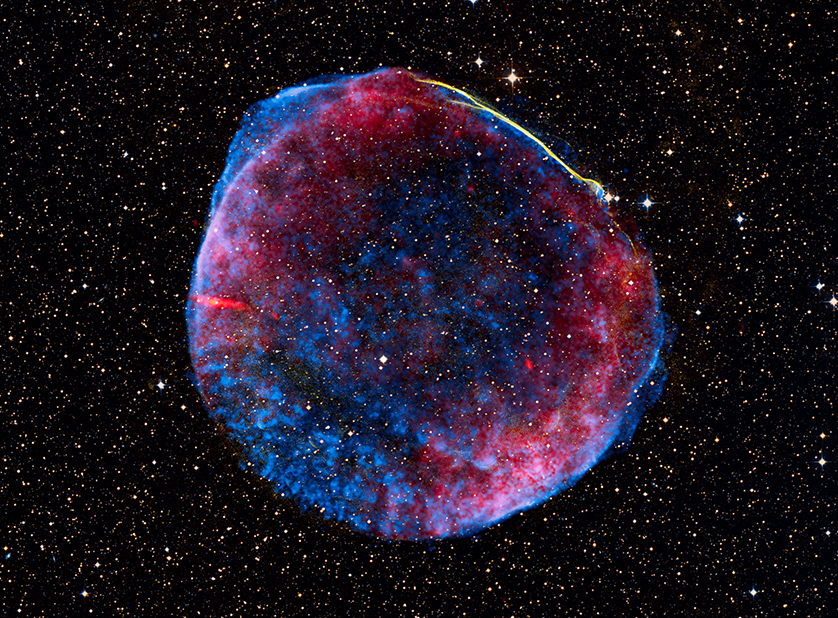
\includegraphics[width=0.65\textwidth]{sn1006c.jpg}
\caption{Composite image of the SN 1006 supernova remnant. X-ray data from NASA’s Chandra X-ray Observatory are in blue.}
\end{figure}

X-ray synchrotron from SNR shocks first established for SN1006.

Is related to loss-limited X-ray synchrotron emission.

We equate the acceleration time with the synchrotron loss-time
\[
\tau_{\rm acc} = \frac{D}{u_s^2} \sim \tau_{\rm syn}
\]
%
as \( \tau_{\rm syn} \propto E^{-1} B^{-2} \)

follows that the max energy for which the two are the same
%
\[
E \sim \frac{u_s^2}{B^2 D} 
\]


\section{The need of a non-linear theory of diffusive shock acceleration}

{\color{red}To be done}

%\newpage
%
%\begin{mdframed}
%We found that the particle accelerated spectrum in case of strong shock follows $n(E) \sim E^{-2}$.  
%%
%In this approach, we have obtained this result explicitly assuming that the system is stationary, which is absurd. In this system the particles gain always energy, so in this case the total energy of a stationary should be infinite.
%
%Let's calculate the total energy of the system by focusing on the relativistic particles only:
%%
%\begin{equation}
%\epsilon_{tot} = \int_{m_p c^2}^{E_{\rm max}} dE \, E \, n(E)  \propto \ln \left( \frac{E_{\rm max}}{m_p c^2} \right)
%\end{equation}
%
%The energy to accelerate this particles cannot be taken anywhere else than from the kinetic energy of the plasma, which energy density is $\rho u^2$.
%
%We can choose $E_{max}$ to mach to $\rho u^2$ (however $E_{max}$ depends on the microphysics of the transport).  The problem here is that this is a \textbf{text particle theory},  where cosmic rays are assumed to behave as test particles and as such they cannot possibly affect the system.  This has as a consequence that the accelerated particles can reach energies comparable to those of the plasma itself.  
%\begin{enumerate}
%\item
%This is a signal that,  in practice, we have to develop a non-linear theory,  \textbf{we cannot have test particles}.  
%\item If we assume $E_{max}$ finite the system cannot be stationary: the energy can only increase.  The only way to avoid this conclusion is to allow the particles to leave the system:
%\begin{equation}
%f(z_0,p)=0
%\end{equation}
%This condition is known as \textbf{free escape boundary condition}. In this case we would obtain that there is an exponential decay for the maximum value of momentum.
%\end{enumerate}
%
%We have studied conservation laws
%\begin{equation}
%\frac{\partial}{\partial z}\left[\rho u^2 +P_{gas}  \right]=0 \implies  \rho u^2 +P_{gas} =\text{constant}
%\end{equation}
%What if our particles affect the system? We have $\rho\sim$eV cm$^{-3}$,  $E_{CR}=1$GeV,  $n=1$cm$^{-3}$ and $n_{CR}=10^{-9}$cm$^{-3}$ (cosmic rays can be neglected from the point of view of conservation of mass).  In the presence of cosmic rays the momentum conservation equation becomes
%\begin{equation}
%\rho u^2 +P_{gas}+P_{CR} =\text{constant}
%\end{equation}
%What happens in the upstream? If we are sitting at the upstream infinity (we call it with a subscript $0$) there are no cosmic rays:
%\begin{equation}
%\begin{aligned}
%\rho_0 u_0^2 +P_{gas,0} &=\rho_1 u_1^2 +P_{gas,1}+P_{CR}\\
%1+\cancel{\frac{P_{gas,0}}{\rho_0 u_0^2}}&=\frac{\rho_1 u_1^2}{\rho_0 u_0^2} +\cancel{\frac{P_{gas,1}}{\rho_0 u_0^2}}+ \frac{P_{CR}}{\rho_0 u_0^2}\\
%1&= \frac{u_1}{u_0}+\xi_{CR}
%\end{aligned}
%\end{equation}
%In the $0$ the cosmic rays are suppressed and we have used
%\begin{equation}
%\frac{P_{gas,0}}{\rho_0 u_0^2}=\frac{c_S^2}{\gamma_g u_0^2}=\frac{1}{\gamma_g M_0^2} \overset{M_0 \gg 1}{\longrightarrow} \ll 1
%\end{equation}
%and $\rho_1 u_1=\rho_0 u_0$.
%\\
%If $\xi_{CR}=0$ we are not accelerating particle.  If $\xi_{CR}\neq 0$
%\begin{equation}
%\frac{u_1}{u_0}=1-\xi_{CR}
%\end{equation}
%So when we are accelerating particles effectively,  plasma in the upstream slows down.  There are no such things as test particles.
%
%We have two processes:
%\begin{enumerate}
%\item
%\textbf{Dynamical action of accelerated particles}: imposing mass and momentum conservation we have found that
%\begin{equation}
%\xi_{CR}\equiv \frac{P_{CR,1}}{\rho_0 u_0^2}=1-\frac{u_1}{u_0}
%\end{equation}
%When particles are accelerated,  the plasma has to slow down.  At low energies particles will have a smaller diffusion coefficient than a high energy particle.  It feels a compression factor $r_1$,  whereas a high energy particle feels the compression factor $r_2$.  So \textbf{the compression factor $r$ depends on momentum}.  \textbf{The power spectrum cannot be a perfect power law}.  At maximum $r=4$,  for lower $r$,  the spectrum becomes steeper.
%\item
%\textbf{Magnetic implication}
%\begin{equation}
%D(p)=\frac{1}{3}r_L(p)v\frac{1}{\mathcal{F}(k)} \implies {\mathcal{F}}(k) \sim \frac{\delta B^2}{B_0^2}\left(k_{res}=\frac{1}{r_L}\right)
%\end{equation}
%The only way to decrease acceleration time is to decrease $D$.  So we have to increase $\delta B$,  we have to create large perturbations.  Remember that in non linear theories the parameters $u$ and $D$ of the transport equation become dependent on $f$ itself.  The action of CR is to slow down the plasma.
%\end{enumerate}
%\end{mdframed}
